\section{The chess theorem}

\begin{theorem}[Von Neumann]
    In the game of chess one and only one of the following alternatives holds:
    \begin{enumerate}
        \item The white has a way to win, no matter what the black does.
        \item The black has a way to win, no matter what the white does.
        \item The white has a way to force at least a draw, no matter what the black does, and the same holds for the black.
    \end{enumerate}
\end{theorem}
\begin{proof}
    Suppose the length of the game is $2K$ so each player has $K$ choices to make.
    Call $a_i$ the move of the White at her $i$-th stage and $b_i$ the one of the Black. 
    The first alternative in the chess theorem can be expressed as
    \[\exists a_1 : \forall b_1 \exists a_2 : \forall b_2 \dots \exists a_K : \forall b_K \implies \text{white wins}\]
    Now suppose this is not true. Then
    \[\forall a_1 \exists b_1 : \forall a_2 : \exists b_2 : \dots \forall a_K : \exists b_K \implies \text{white does not win}\]
    But this means exactly that Black has the possibility to get at least a draw.
\end{proof}
If White does not have a strategy to win no matter what Black does, then Black has the possibility to get at least the draw.
Symmetrically, if Black does not have a strategy to win no matter what White does, then White has the possibility to get at least the draw
Thus if the first and the second alternatives in the chess theorem are not true, necessarily the third one is true. 

\subsection*{Von Neumann theorem extension}
The von Neumann theorem applies to every finite game of perfect information where the possible result is either the victory of one player or a tie. Thus the following corollary holds:
\begin{corollary}
    Consider a finite perfect information game with two players, where the only possible outcomes are the victory of one or the other player. 
    Then one and only one of the following alternative holds:
    \begin{enumerate}
        \item The first player can win, no matter what the second one does.
        \item The second player can win, no matter what the first one does.
    \end{enumerate}
\end{corollary}
The possible solutions of a game are the follwing: 
\begin{itemize}
    \item Very weak solution: the game has a rational outcome, but it is inaccessible, like in chess.
    \item Weak solution: the outcome of the game is known, but how to get to it is not (in general).
    \item Solution: it is possible to provide an algorithm to find a solution.
\end{itemize}
\begin{example}
    Consider the game of chomp.
    In this game we have a grid in which each player can remove a tile with all the others on the right and above it. 
    In this game we have a solution if the grid is a square, and a weak solution if the grid is rectangular.
    In the latter case we may have the following situation: 
    \begin{figure}[H]
        \centering
        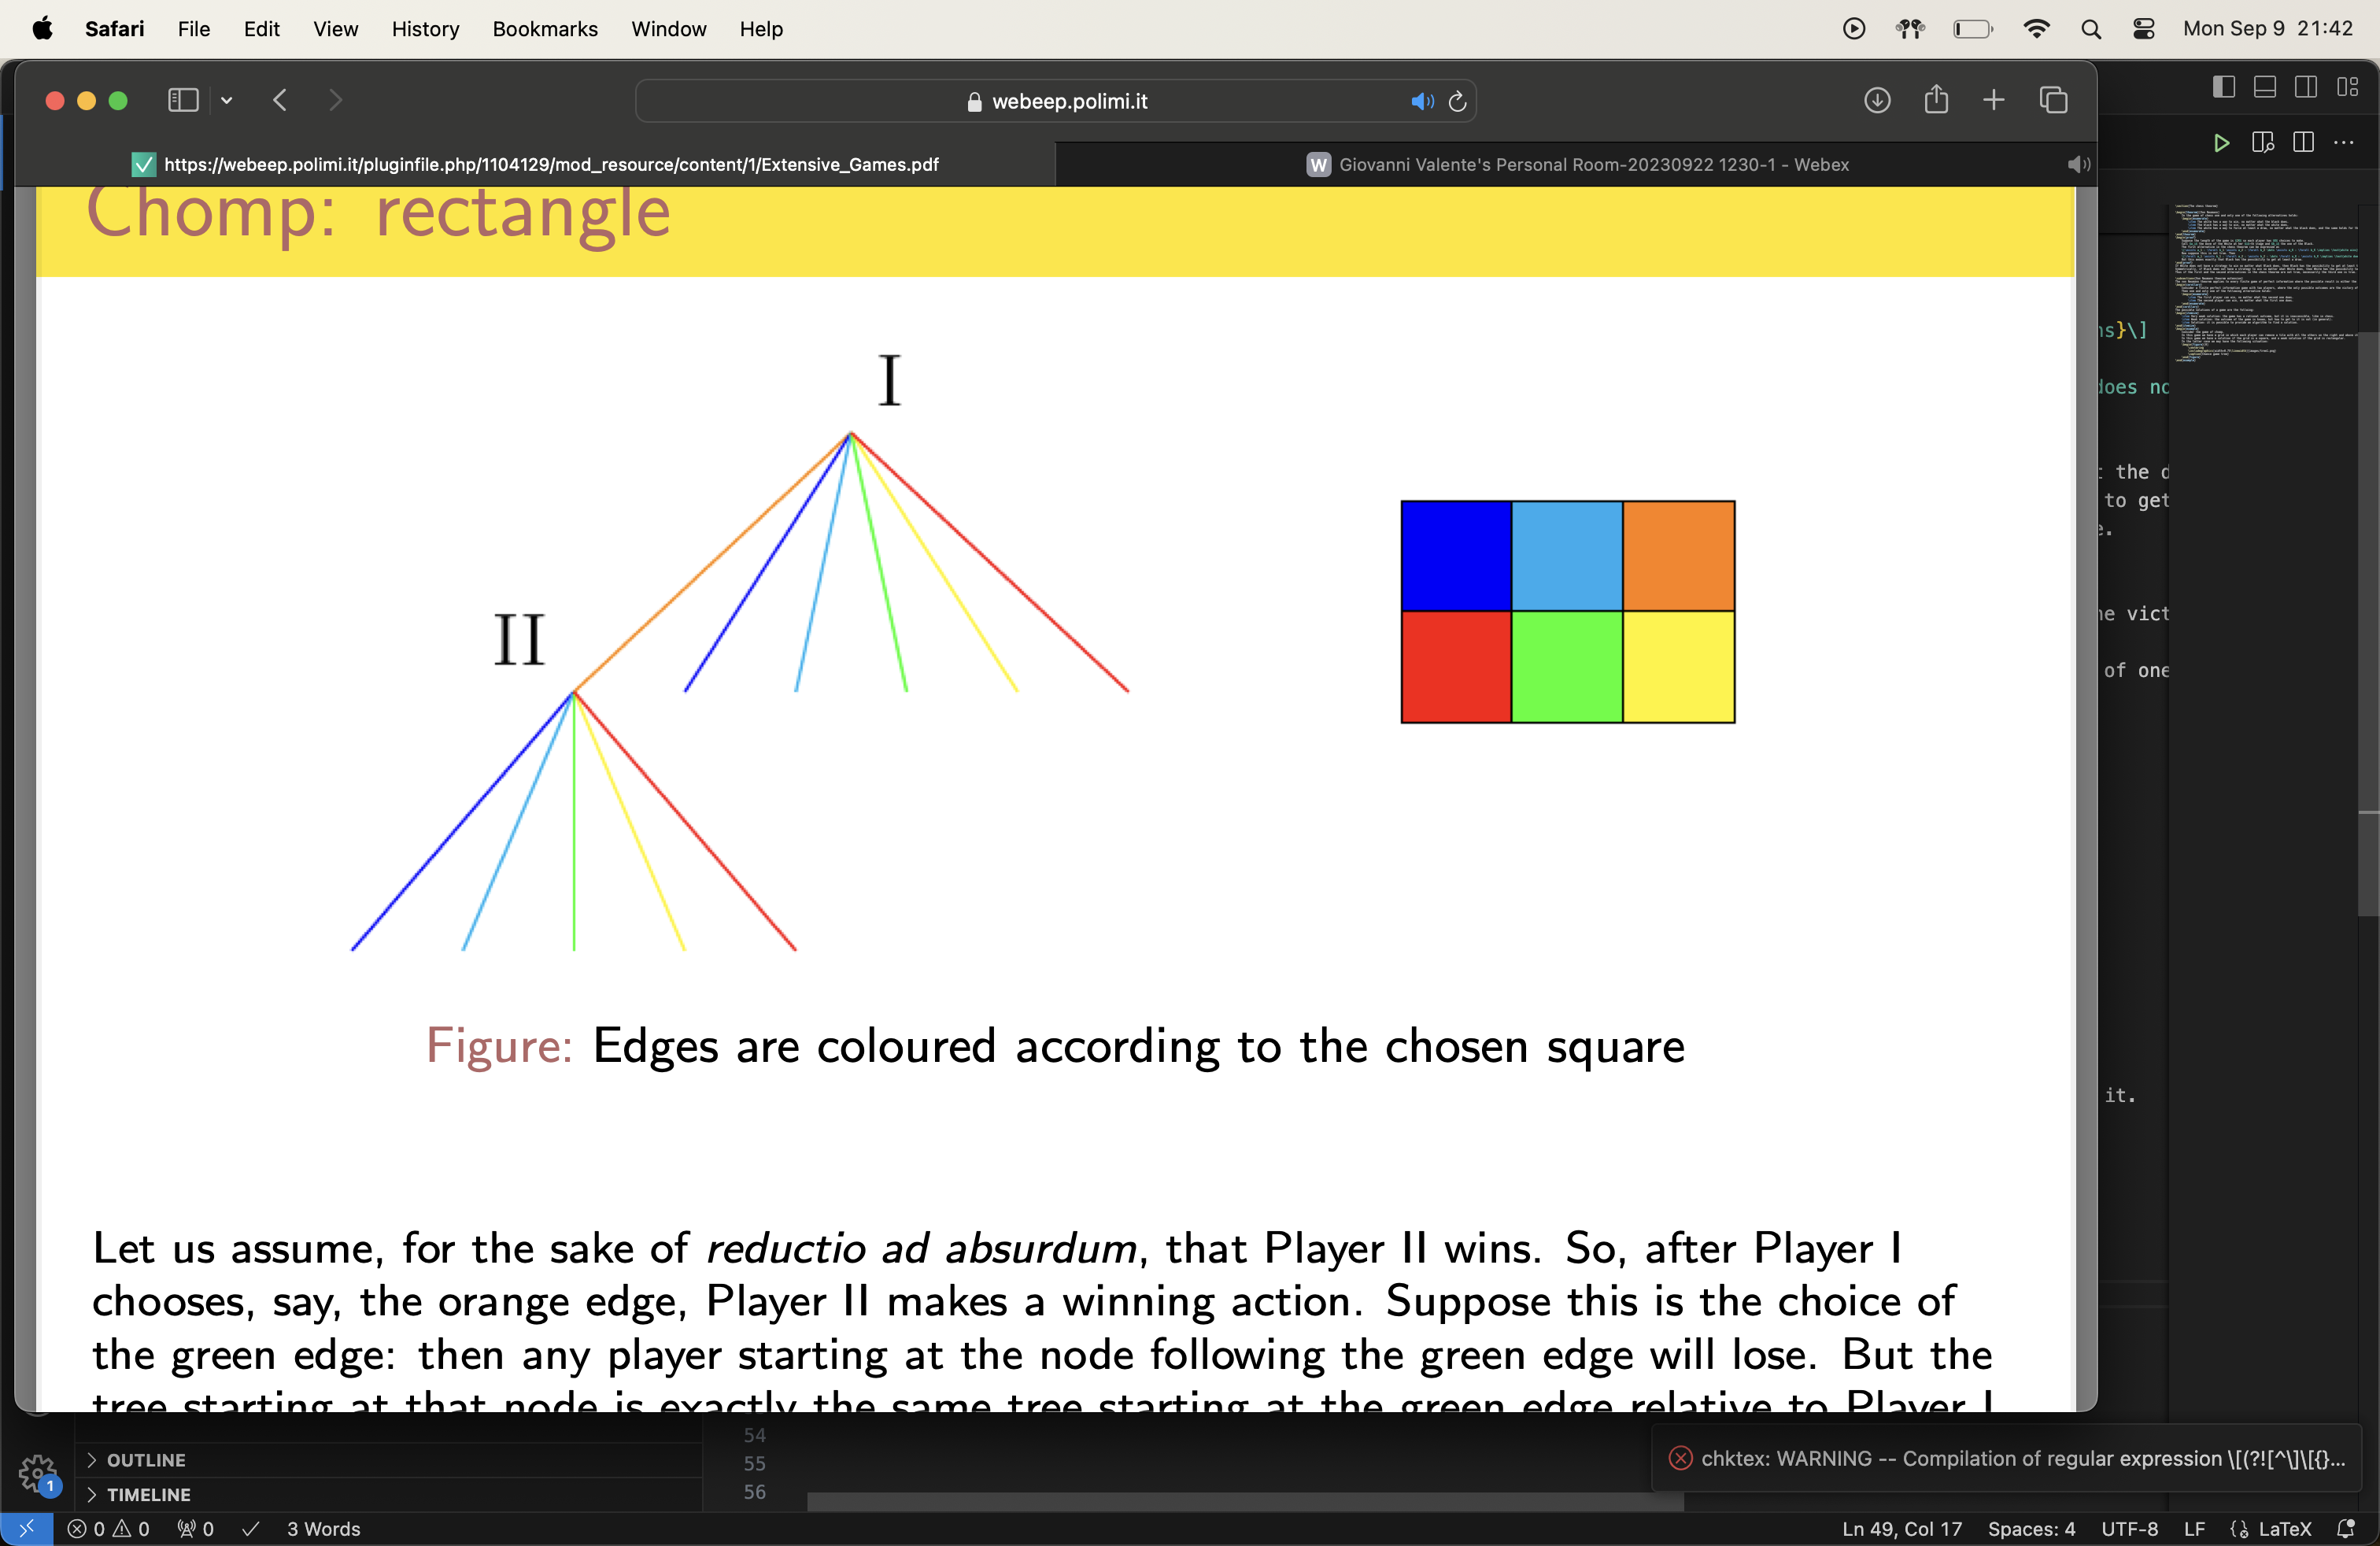
\includegraphics[width=0.75\linewidth]{images/chomp.png}
        \caption{Rectangular chomp}
    \end{figure}
    Let us assume, for the sake of reductio ad absurdum, that Player II wins. So, after Player I
    chooses, say, the orange edge, Player II makes a winning action. Suppose this is the choice of
    the green edge: then any player starting at the node following the green edge will lose. But the
    tree starting at that node is exactly the same tree starting at the green edge relative to Player I.
    Thus Player I has a move available that guarantees victory, whereby Player II would have to lose.
    Since we derived a contradiction, the original assumption must be false: it is Player I that wins!
\end{example}







